% Figura cuerpo B3: el mismo tablero con parámetros opuestos: (a) mundo de la Síntesis; (b) mundo monetarista
\documentclass[tikz,border=3pt]{standalone}
\usepackage[T1]{fontenc}
\usepackage[utf8]{inputenc}
\usetikzlibrary{arrows.meta,calc,positioning}
\begin{document}
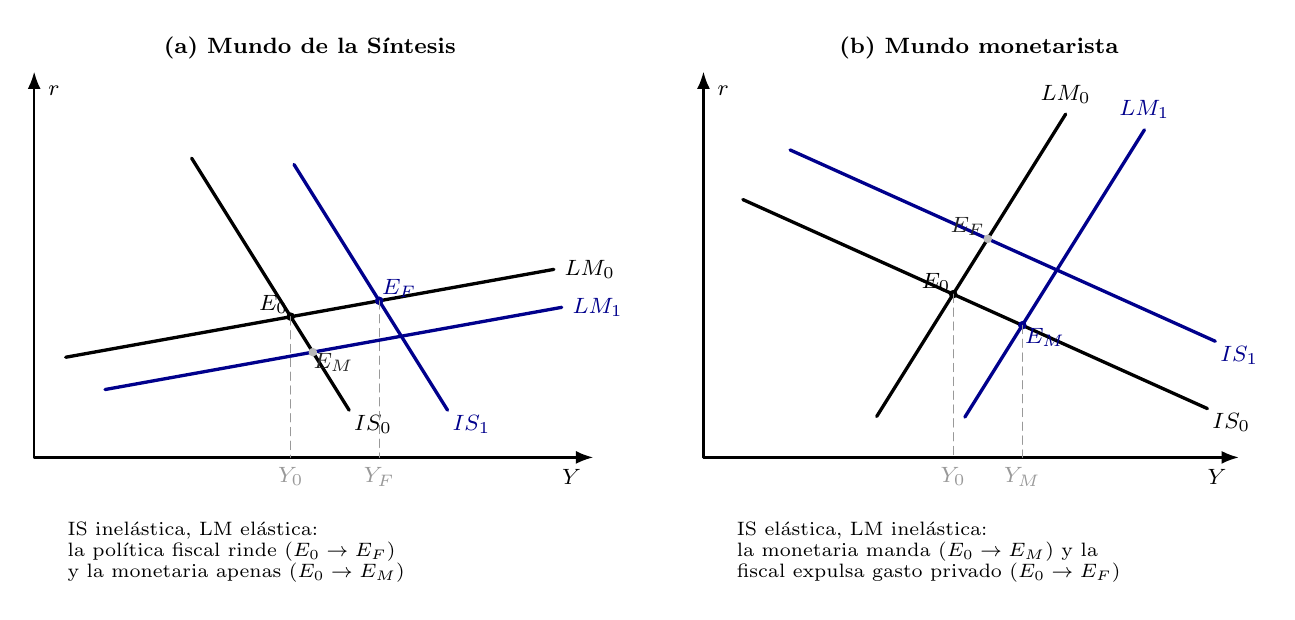
\begin{tikzpicture}[>={Latex[length=2.2mm]}, line cap=round, font=\footnotesize,
  eje/.style={->, thick},
  curva/.style={very thick},
  nueva/.style={very thick, blue!55!black},
  guia/.style={densely dashed, gray!80},
  pto/.style={circle, fill=black, inner sep=1.1pt}]
  % ---------- Panel (a): mundo de la Síntesis ----------
  \node[font=\footnotesize\bfseries] at (3.5,5.2) {(a) Mundo de la Síntesis};
  \draw[eje] (0,0) -- (7.1,0) node[below left=1pt]{$Y$};
  \draw[eje] (0,0) -- (0,4.9) node[below right=2pt]{$r$};
  \draw[curva] (0.4,1.272) -- (6.6,2.388) node[right]{$LM_0$};
  \draw[nueva] (0.9,0.862) -- (6.7,1.906) node[right]{$LM_1$};
  \draw[curva] (2.0,3.8) -- (4.0,0.6) node[below right=-3pt]{$IS_0$};
  \draw[nueva] (3.3,3.72) -- (5.25,0.6) node[below right=-3pt]{$IS_1$};
  \node[pto] (E0) at (3.258,1.787) {};
  \node[above left=-2pt of E0, inner sep=1pt] {$E_0$};
  \node[pto, fill=blue!55!black] (EF) at (4.382,1.989) {};
  \node[above right=-2pt of EF, inner sep=1pt, blue!55!black] {$E_F$};
  \node[pto, fill=gray!55] (EM) at (3.539,1.337) {};
  \node[below right=-3pt of EM, inner sep=1pt, gray!30!black] {$E_M$};
  \draw[guia] (3.258,1.787) -- (3.258,0) node[below]{$Y_0$};
  \draw[guia] (4.382,1.989) -- (4.382,0) node[below]{$Y_F$};
  \node[align=left, anchor=north west] at (0.3,-0.7) {\scriptsize IS inelástica, LM elástica:\\[-2pt]\scriptsize la política fiscal rinde ($E_0\to E_F$)\\[-2pt]\scriptsize y la monetaria apenas ($E_0\to E_M$)};
  % ---------- Panel (b): mundo monetarista ----------
  \begin{scope}[xshift=8.5cm]
    \node[font=\footnotesize\bfseries] at (3.5,5.2) {(b) Mundo monetarista};
    \draw[eje] (0,0) -- (6.8,0) node[below left=1pt]{$Y$};
    \draw[eje] (0,0) -- (0,4.9) node[below right=2pt]{$r$};
    \draw[curva] (2.2,0.52) -- (4.6,4.36) node[above]{$LM_0$};
    \draw[nueva] (3.32,0.512) -- (5.6,4.16) node[above]{$LM_1$};
    \draw[curva] (0.5,3.275) -- (6.4,0.62) node[below right=-3pt]{$IS_0$};
    \draw[nueva] (1.1,3.905) -- (6.5,1.475) node[below right=-3pt]{$IS_1$};
    \node[pto] (F0) at (3.171,2.073) {};
    \node[above left=-2pt of F0, inner sep=1pt] {$E_0$};
    \node[pto, fill=gray!55] (FF) at (3.61,2.776) {};
    \node[above left=-2pt of FF, inner sep=1pt, gray!30!black] {$E_F$};
    \node[pto, fill=blue!55!black] (FM) at (4.049,1.678) {};
    \node[below right=-2pt of FM, inner sep=1pt, blue!55!black] {$E_M$};
    \draw[guia] (3.171,2.073) -- (3.171,0) node[below]{$Y_0$};
    \draw[guia] (4.049,1.678) -- (4.049,0) node[below]{$Y_M$};
    \node[align=left, anchor=north west] at (0.3,-0.7) {\scriptsize IS elástica, LM inelástica:\\[-2pt]\scriptsize la monetaria manda ($E_0\to E_M$) y la\\[-2pt]\scriptsize fiscal expulsa gasto privado ($E_0\to E_F$)};
  \end{scope}
\end{tikzpicture}
\end{document}
